\documentclass[../main]{subfiles}

\begin{document}

\letAnjana

\subsection{Learning the Fundamentals of Fusion 360-3D CAD Modelling}

The aim is to get familiar with the interface, sketching tools, modeling
operations, and assembly creation processes to later apply them in mechanical
design tasks such as modeling linear rails, sensor holders, and camera mounts.

\paragraph{} Learned to create a simple toy block, which covered essential
tools like sketching, extruding, and patterning.

\begin{figure}
    \centering
    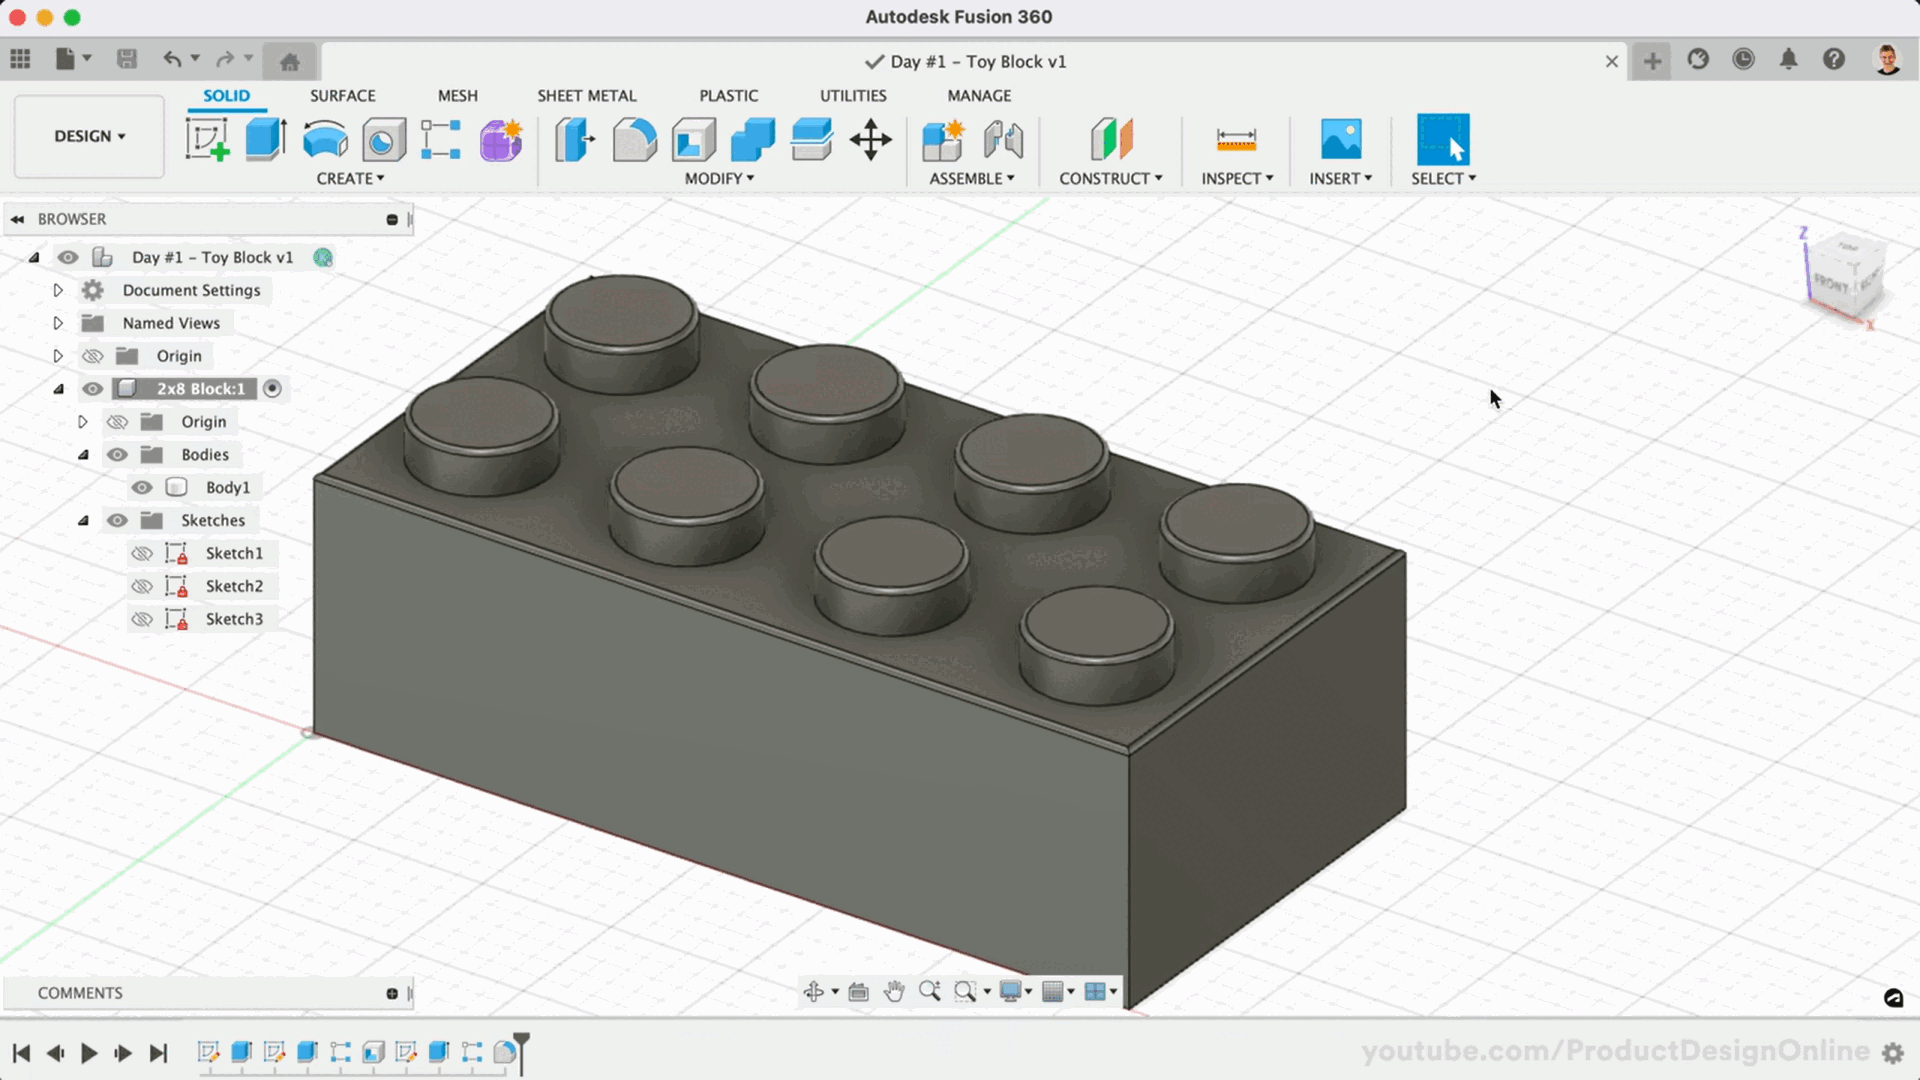
\includegraphics[width=0.5\textwidth,height=.2\textheight]{ss1.png}
    \caption{Designing of sample toy block} \label{pm}
\end{figure}

\paragraph{} Created a glass soda bottle, covering techniques like inserting a
reference image, using the Revolve tool, and applying a glass appearance.

\begin{figure}
    \centering
    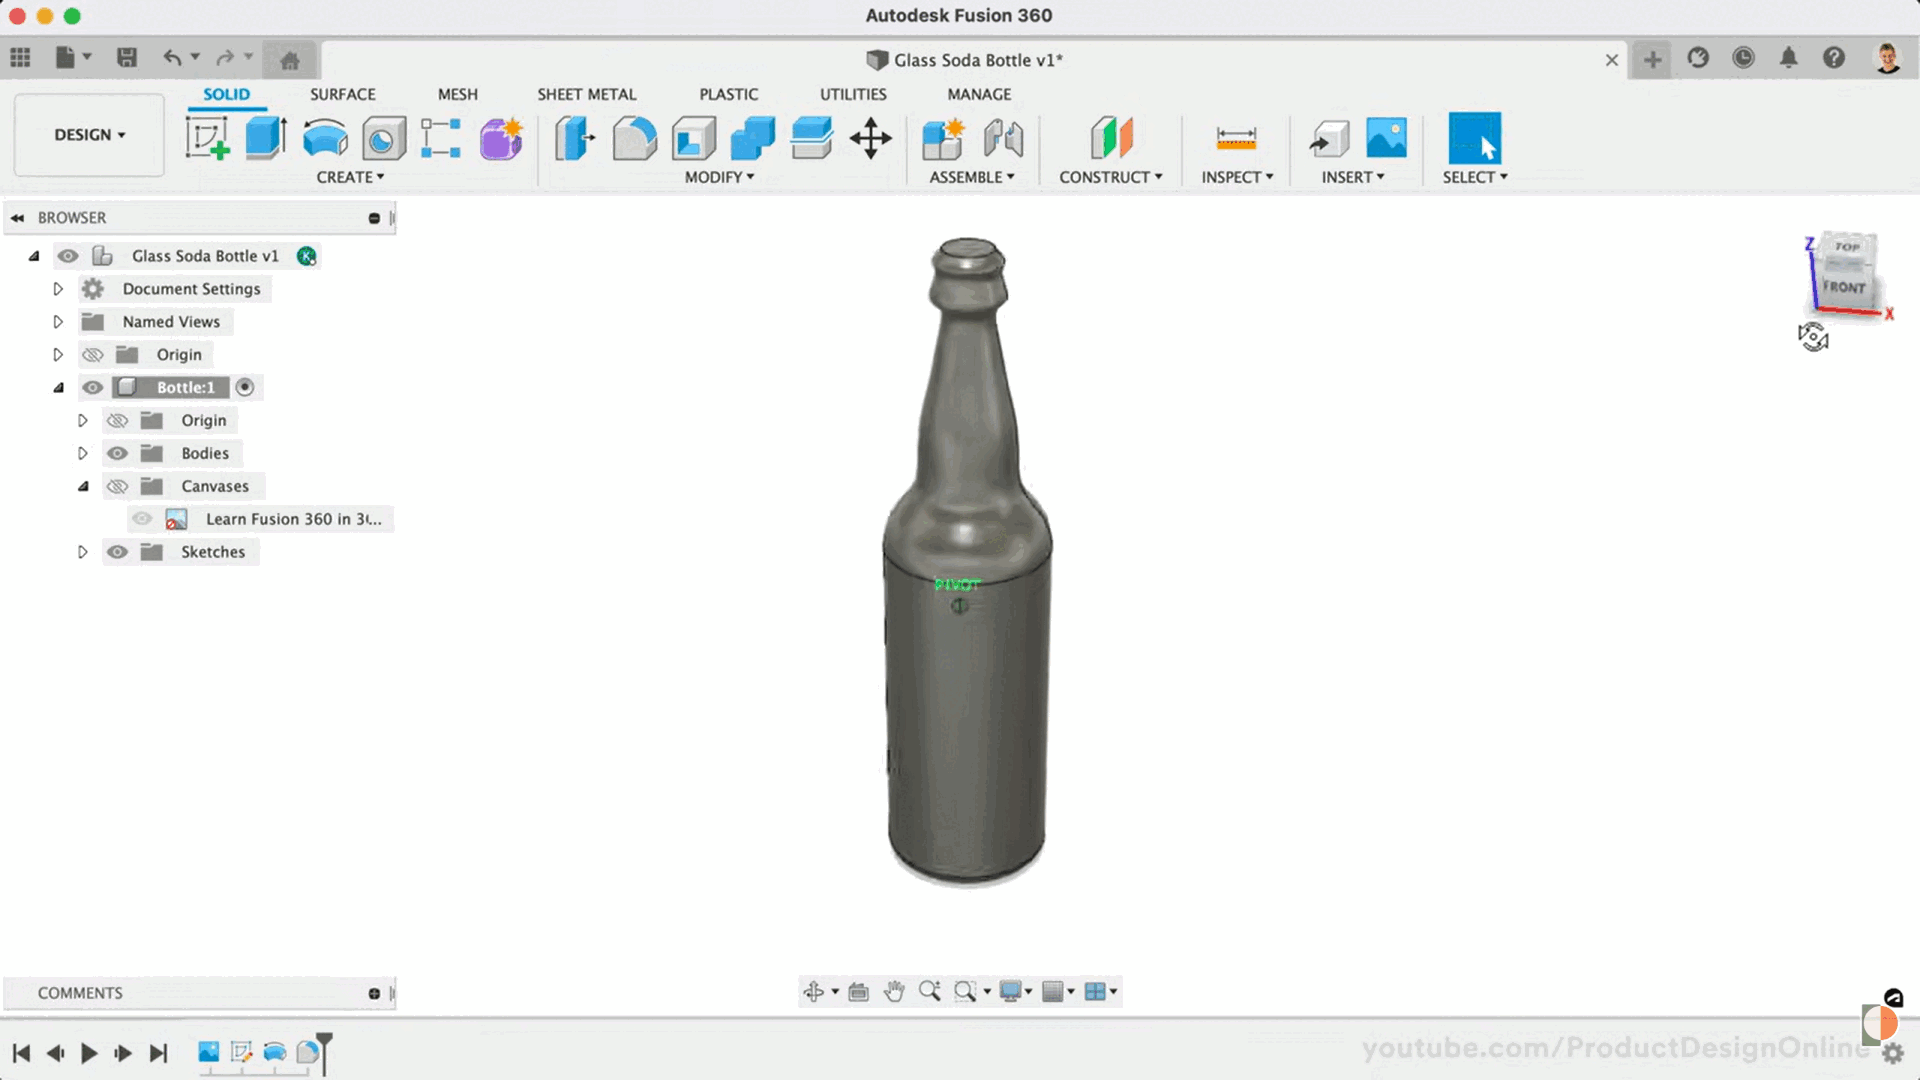
\includegraphics[width=0.5\textwidth,height=.2\textheight]{ss2.png}
    \caption{Designing of sample glass bottle} \label{pm}
\end{figure}

\end{document}
